\chapter{Hyperbolic representation learning}\label{hrl}
We now combine the notions discusses in \Cref{grl} and \Cref{hyperbolic} to learn representations of hyperbolic spaces. We initially look at how shallow embeddings have been implemented in hyperbolic space., and we then expand on the concept of graph neural networks in hyperbolic space.

\section{Poincaré embeddings for hierarchical learning}
We analyze an approach for learning hierarchical representations of data by embedding them into a hyperbolic space in a shallow manner~\cite{nickel2017poincare}. This technique is based on the assumption that there exists a latent hierarchy in which the data can be organized. Nevertheless, there is no direct access to information about the hierarchy, such as ordered input pairs. Thus the task of inferring the hierarchical relationships is fully unsupervised. 

\paragraph{Model choice}
Seen the nature of the task and the considerations brought out in \Cref{sec:hyperbolicAndTrees} it is useful to project the data into hyperbolic space. The Poincaré ball model is favoured since it is well-suited for gradient-based optimization. Also, using the ball in $d$-dimensions allows to learn multiple latent hierarchies that co-exist in a dataset. 

As seen in \Cref{eq:poincareDistance} the distance within the Poincaré ball changes smoothly with respect to the location of $p$ and $q$. This locality property of the Poincaré distance is key for finding continuous embeddings of hierarchies. For instance, by placing the root node of a tree at the origin of the Poincaré ball $\B^d$ it would have a relatively small distance to all other nodes as its Euclidean norm is zero. On the other hand, leaf nodes can be placed close to the boundary of the Poincaré ball as the distance grows very fast between points with a norm close to one. This is made evident when observing \Cref{fig:radialTree} and imagining the tree projected onto a hyperbolic sheet, as shown in \Cref{fig:hyperboloidToPoincareBall}. Furthermore, \Cref{eq:poincareDistance} is symmetric and the hierarchical organization of the space is solely determined by the distance of points to the origin. Due to this self-organizing property, \Cref{eq:poincareDistance} is applicable in an unsupervised setting where the hierarchical order of objects is not specified in advance. 

\paragraph{Optimization}
We assume we are given a problem-specific loss function $\mathcal{L}$ which encourages semantically similar objects to be close in the embedding space according to their Poincaré distance. Since the Poincaré ball has a Reimannian manifold structure, we can minimize the loss using \term{Reimannian Stochastic  Gradient Descent} (\term{RSGD})~\cite{bonnabel2013RSGD} (or other Reimannian optimization methods). The usual update on gradient $w$ at time $t$ is replaced with the following update rule:

\begin{equation}
    w_{t+1} = \exp_{w_t}(-\eta_t\nabla_R\mathcal{L}).
\end{equation}
Here $\exp_{w_t}$ stands for the exponential map\footnote{When the exponential map is not easy to compute one can use a retraction. This map $R_w:\mathcal{T}_w\Mcal\to\Mcal$ is a first-order approximation of the exponential such that $d(exp_w(v), R_w(v))=\|v\|_2+O(\|v\|^2_2)$} at point $w_t$ towards $\mathbb{B}^d$, $\eta_t$ denotes the learning rate at time $t$, and $\nabla_R \mathcal{L} \in \mathcal{T}_{w}\mathbb{B}^d$ indicates the Riemannian gradient of $\mathcal{L}$, where $\mathcal{T}_{w}\mathbb{B}^d$ is the tangent space of a point $w \in \mathbb{B}^d$.  

\section{Hyperbolic Graph Neural Networks (HGNN)}
As we discussed in \Cref{sec:gnn}, graph neural networks allow to build inductive representations of the nodes in a graph. This technique involves a series of basic operations, like message passing on a set of nodes in a given space. While such operations are well-understood in Euclidean space, their counterparts in non-Euclidean space are non-trivial. We generalize the notion of a graph neural network so that the architecture operates on Reimannian manifolds, resulting in a \term{Hyperbolic Graph Neural Network} (\term{HGNN})~\cite{liu2019HGNN}. Since the tangent space of a point on Reimannian manifolds is always Euclidean---or a subset of Euclidean space---functions with trainable parameters can be defined on the tangent space using the exponential and logarithmic maps (Equations~\eqref{eq:log_poincareBall} and \eqref{eq:exp_poincareBall} in the case of the Poincaré ball model). Taking as baseline the update for a basic GNN with self-loops (recall \Cref{eq:basicGNNgraphlevelselfLoop}), in a HGNN the information propagates for each node $u \in V$ as follows:

\begin{equation}\label{eq:HGNNgraphlevel}
    \mathbf{h}^{(\ell)}_u = \sigma\left(\exp_p\left(\sum_{v\in\mathcal{N}(u)}\left(\mathbf{A} + \mathbb{I}_{|V|}\right)\mathbf{W}^{(\ell)}\log_p\left(\mathbf{h}^{(\ell-1)}_v\right)\right)\right).
\end{equation}

At layer $\ell$ for each of $u$'s neighbours $v\in\mathcal{N}(u)$ we map their representation $\mathbf{h}^{(\ell)}_v\in \Mcal$ to the tangent space of a chosen point $p\in \Mcal$ using the logarithmic map $\log_p(\cdot)$. As in \Cref{eq:basicGNNgraphlevelselfLoop} $\mathbf{A}$ is the graph adjacency matrix and $\mathbf{W}^{(\ell)}$ are the trainable parameters of the layer. The exponential map $\exp_p(\cdot)$ is then used to map the linearly transformed tangent vector back to the manifold. The exponential map is applied before the activation function $\sigma$ to avoid the logarithmic and exponential maps cancelling out when nested between steps. 

\paragraph{Activation functions}
When applying the non-linear activation function on a manifold $\Mcal$ we need to assure that it is \term{manifold preserving} such that $\sigma: \Mcal\to\Mcal$. In the case of the Poincaré ball model it is sufficient to employ pointwise non-linearities which are norm decreasing, so that $|\sigma(x)|\leq |x|$. This is true for ReLU and LeakyReLU, for which $\|\sigma(\mathbf{x})\|\leq \|\mathbf{x}\|$, ensuring that $\sigma: \B\to \B$. For other hyperbolic models it is sufficient to use the stereographic projection and its inverse, detailed in Equations~\eqref{eq:stereographicProjection} and \eqref{eq:inverseStereographicProjection}.

\section{Hyperbolic Graph Convolutional Neural Networks (HGCN)}
Similar to HGNN, core graph neural network operations in \term{Hyperbolic Graph Convolutional Networks} (\term{HGCN}s)~\cite{chami2019HGCN} are in hyperbolic space. This algorithm expands HGNN in the following aspects.

\begin{description}
    \item[Input mapping to hyperbolic space] Since input features are often Euclidean, one derives a mapping from Euclidean features to hyperbolic space.
    \item[Hyperbolic message-passing] An adaptation to hyperbolic manifolds of the message update equation, by tweaking the feature transform component (\Cref{eq:featureTransform}) and the message passing step (\Cref{eq:neighAgg}).
    \item[Trainble curvature] At different layers of HGCN the feature transformations in hyperbolic spaces are applied at different trainable curvatures to learn low-distortion hyperbolic embeddings.
\end{description}

To maintain conformity with~\cite{chami2019HGCN} we refer to the hyperboloid model, whilst specifying that the same considerations apply to the Poincaré ball model.

\paragraph{Notation}
Before delving into the details of the HGCN architecture we add some detail to a few quantities presented in \Cref{sec:hyperboloidModel}. 

We generalize the exponential and logarithmic maps for the hyperboloid model (Equations~\eqref{eq:log_hyperboloid} and \eqref{eq:exp_hyperboloid}) having constant negative curvature $\frac{1}{\kappa}$ by defining them as follows.
\begin{align}
    \exp_p^\kappa(v) &= \cosh\left(\frac{\|v\|_\Lcal}{\sqrt{\kappa}}\right)p + \sqrt{\kappa}\sinh\left(\frac{\|v\|_\Lcal}{\sqrt{\kappa}}\right) \frac{v}{\|v\|_\Lcal} \label{eq:expk_hyperboloid}\\
    \log_p^\kappa(y) &= d_{\Lcal}^\kappa(p,y)\frac{y + \frac{1}{\kappa}\langle p,y \rangle_{\Lcal}p}{\|y + \frac{1}{\kappa}\langle p,y \rangle_{\Lcal}p\|_{\Lcal}} \label{eq:logk_hyperboloid}
\end{align}
In this case the intrinsic distance between two points $p, q\in\Hy^{d,K}$ is given by the following equation (refer to \Cref{eq:distance_hyperboloid}):
\begin{equation*}
    d_{\Hy^{d,\kappa}}(p, q) = \sqrt{K}\text{arcosh}(-\langle p, q \rangle_\Lcal).
\end{equation*}

\subsection{Input mapping to hyperbolic space}
The input features of neural networks are typically in Euclidean space, thus one first maps them into the Reimannian manifold through the exponential map centered in the origin of the manifold. Subsequently the point on the hyperbolic space is projected onto the chosen model.

Let $\mathbf{x}^{(0), E}\in\R^d$ be input Euclidean features on the graph edges. Let $\mathbf{o}=(\sqrt{\kappa}, 0, \dots,0)\in \Hy^{d,\kappa}$ denote the origin in $\Hy^{d,\kappa}$, which we use as a reference point to perform tangent space operations. Since we have that $\langle({0},\mathbf{x}^{(0), E}), \mathbf{o}\rangle_\Lcal=\mathbf{o}$, we interpret $({0},\mathbf{x}^{(0)})$ as a point in $\mathcal{T}_\mathbf{o}\Hy^{d,\kappa}$ (recall the definition of tangent spaces in the hyperbolic model in \Cref{eq:tangentSpace}). We then use the exponential map described in \Cref{eq:expk_hyperboloid} to map the input features to the hyperbolic space.
\begin{equation}
    \exp_{\mathbf{o}}^\kappa(\mathbf{x}^{(0), E}) = \left(\sqrt{\kappa}\cosh\left(\frac{\|\mathbf{x}^{(0), E}\|_2}{\sqrt{\kappa}}\right), \sqrt{\kappa}\sinh\left(\frac{\|\mathbf{x}^{(0), E}\|_2}{\sqrt{\kappa}}\right)\frac{\mathbf{x}^{(0), E}}{\|\mathbf{x}^{(0), E}\|_2}\right)
\end{equation}

\subsection{Feature transform in hyperbolic space}
The feature transform used in the message-passing step for the basic GNN (\Cref{eq:featureTransform}) is used to map the embedding space of a layer to the one in the next layer. Since there is no notion of vector space structure in hyperbolic space one can leverage the exponential and logarithmic maps outlined in Equations~\eqref{eq:expk_hyperboloid} and \eqref{eq:logk_hyperboloid} to perform Euclidean transformations on the tangent space $\mathcal{T}_\mathbf{o}\Hy^{d,\kappa}$. 

The feature transform step requires a multiplication of the embedding vector by a weight matrix, followed by a (optional) bias translation. To compute matrix vector multiplication we first use the logarithmic map to project hyperbolic points $\mathbf{x}$ to $\mathcal{T}_\mathbf{o}\Hy^{d,\kappa}$. This implies that the matrix $\mathbf{W}$ representing the transform is defined on the Euclidean tangent space. We then project the transformed vector in the tangent space back to the manifold using the exponential map. So, the hyperboloid matrix multiplication is defined as:
\begin{equation*}
    \mathbf{W} \otimes^\kappa \mathbf{x} = \exp_{\mathbf{o}}^\kappa\left(\mathbf{W}\log_{\mathbf{o}}^\kappa(\mathbf{x})\right).
\end{equation*}
Assuming that $\mathbf{W} \in \R^{d}\times d'$, the function $\log_{\mathbf{o}}^\kappa(\cdot)$ is on $\Hy^{d}$ and $\exp_{\mathbf{o}}^\kappa(\cdot)$ is on $\Hy^{d'}$. 

To perform bias addition one can define $\mathbf{b}$ as an Euclidean vector located on the tangent space $\mathcal{T}_\mathbf{o}\Hy^{d,\kappa}$ as done for the HNN model~\cite{ganea2018HNN}. Then one parallel transports the bias vector to the hyperbolic point of interest and maps it to the manifold. If $P_{\mathbf{o}\to \mathbf{x}}^\kappa (\cdot)$ is the parallel transport from $\mathcal{T}_\mathbf{o}\Hy^{d,\kappa}$ to $\mathcal{T}_{\mathbf{x}}\Hy^{d,\kappa}$, the hyperboloid bias addition step is as such:
\begin{equation*}
    \mathbf{x} \oplus^\kappa \mathbf{b} = \exp_{\mathbf{x}}^\kappa\left(P_{\mathbf{o}\to \mathbf{x}}^\kappa\left(\log_{\mathbf{o}}^\kappa(\mathbf{b})\right)\right).
\end{equation*}

\subsection{Neighbourhood aggregation in hyperbolic space}
As seen in \Cref{sec:gnn} regarding GNNs, the neighbourhood aggregation step (\Cref{eq:neighAgg}) is crucial to capture neighbourhood structures and features. The analogue of mean aggregation in Euclidean GNNs (\Cref{eq:aggregateBase}) in hyperbolic space is the Fréchet mean~\cite{frechet1948elements}, which alas has no closed form solution. Therefor, the authors of HGCN perform aggregation in tangent spaces using hyperbolic attention.

\subsubsection{Attention-based aggregation}
Attention in GNNs learns a notion of neighbours' importance and aggregates neighbours' messages accordingly, as discussed in \Cref{sec:neighbourhoodAttention}. However, attention on Euclidean embeddings does not take into account the possible hierarchical nature of graphs. Thus, the need for hyperbolic attention-based aggregation. 

Given a pair of hyperbolic embeddings $(\mathbf{x}_i, \mathbf{x}_j)$, one first maps them to the tangent space to the origin to compute attention weights $w_{ij}$ with concatenation and Euclidean Multi-layer Perceptron (MLP). Then the nodes' representations are averaged, like in the basic GNN. The aggregation step is formalized as:
\begin{equation*}
    \text{AGGREGATE}^\kappa(\mathbf{x})_i = \exp_{\mathbf{x}_i}^\kappa\left(\sum_{j\in\mathcal{N}(i)}w_{ij}\log_{\mathbf{x}_i}^\kappa\left(\mathbf{x}_j\right)\right)
\end{equation*}
and the weights are computed as:
\begin{equation*}
    w_{ij} = \text{softmax}\left(\text{MLP}\left(\log_{\mathbf{o}}^\kappa(\mathbf{x}_i) \left|\right| \log_{\mathbf{o}}^\kappa\left(\mathbf{x}_j\right)\right)\right).
\end{equation*}

In this way the aggregation is directly performed in the tangent space for each point, as this is where the Euclidean approximation is best. This approach is schematized in \Cref{fig:HGCNaggregation}: the message is first mapped to the tangent space, then the aggregation is performed in the tangent space and finally the result is mapped back to the hyperbolic space.

\begin{figure}
  \centering
  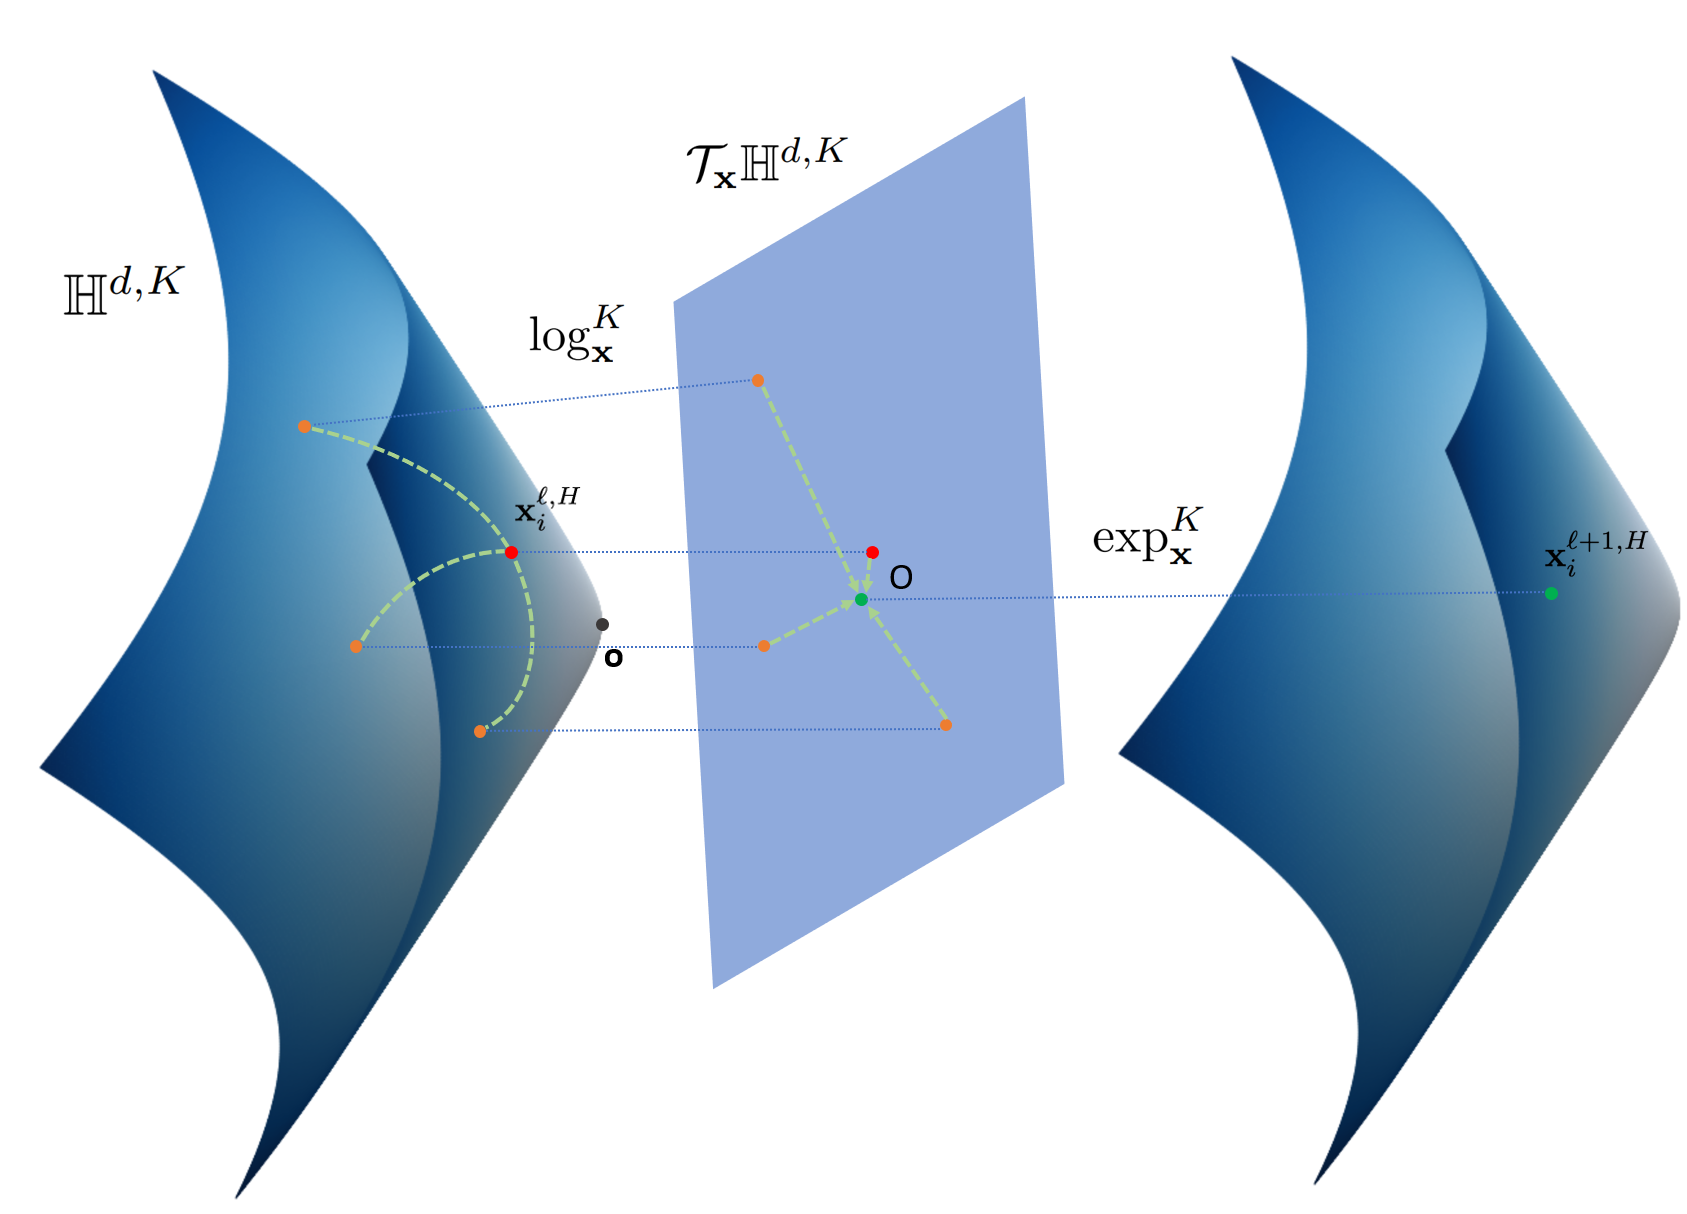
\includegraphics[width=0.7\textwidth]{figs/arch.png}

   \caption{HGCN neighbourhood aggregation~\cite{chami2019HGCN}.}
  \label{fig:HGCNaggregation}
\end{figure}

\subsubsection{Non-linear activation with different curvatures}
Analogous to Euclidean aggregation (\Cref{eq:aggregateBase}) HGCN uses a non-linear activation function $\sigma(\cdot)$ such that $\sigma(0)=0$ to learn non-linear transformations. Given hyperbolic curvatures $-\frac{1}{\kappa^{(\ell-1)}}$ and $-\frac{1}{\kappa^{(\ell)}}$ at layers $\ell-1$ and $\ell$ respectively, the authors introduce a hyperbolic non-linear activation $\sigma^{\otimes^{\kappa^{(\ell-1)}, \kappa^{(\ell)}}}$ for different curvatures. This step is crucial as it allows to smoothly vary curvature at each layer. More concretely, HGCN applies the Euclidean non-linear activation to $\mathcal{T}_\mathbf{o}\Hy^{d,\kappa^{(\ell)}}$ and then maps the result back to $\Hy^{d,\kappa^{(\ell)}}$:
\begin{equation*}
    \sigma^{\otimes^{\kappa^{(\ell-1)}, \kappa^{(\ell)}}}(\mathbf{x}) = \exp_{\mathbf{o}}^{\kappa^{(\ell)}}\left(\sigma\left(\log_{\mathbf{o}}^{\kappa^{(\ell-1)}}(\mathbf{x})\right)\right).
\end{equation*}

Note that in order to apply the exponential map, points must be located in the tangent space at the north pole. Fortunately, tangent spaces of the north pole are shared across hyperboloid manifolds of the same dimension that have different curvatures.

\subsection{HGCN architecture}
Having introduced the building blocks of HGCN we summarize the model architecture in the following algorithm.
\begin{algorithm}
    \caption*{HGCN architecture}
    \begin{algorithmic}
    \State \textbf{Input:} Graph $G=(V, E)$, Euclidean features $(\mathbf{x}^{(0), E})_{u\in V}$
    \State 
    \State $\mathbf{x}^{(0)}_u = \exp_{\mathbf{o}}^{\kappa^{(0)}}(\mathbf{x}^{(0)}_u)$ \Comment{{\footnotesize Map Euclidean features to hyperbolic space}}
    \For{each layer $\ell = 1$ to $L$}
        \For{each node $u \in V$}
            \State $\mathbf{h}^{(\ell)}_u = (\mathbf{W}^{(\ell)} \otimes^{\kappa^{(\ell-1)}} \mathbf{x}^{(\ell-1)}_u) \oplus^{\kappa^{(\ell-1)}} \mathbf{b}^{(\ell)}$ \Comment{{\footnotesize Hyperbolic feature transform}}
            \State $\mathbf{y}^{(\ell)}_u = \text{AGG}^{\kappa^{(\ell-1)}}(\mathbf{h}^{(\ell)})_u$ \Comment{{\footnotesize Attention-based neighborhood aggregation}}
            \State $\mathbf{x}^{(\ell)}_u = \sigma^{\otimes^{\kappa^{(\ell-1)}, \kappa^{(\ell)}}}(\mathbf{y}^{(\ell)}_u)$ \Comment{{\footnotesize Non-linear activation with different curvatures}}
        \EndFor
    \EndFor
    \State
    \State \textbf{Output:} Hyperbolic node embeddings $(\mathbf{x}^{(L)})_{u\in V}$
    \end{algorithmic}
    \label{alg:HGCN}
\end{algorithm}

The returned node embeddings can then be used for node classification or link prediction tasks (recall \Cref{sec:graphLearningProblems}).

\paragraph{Node classification}
For node classification tasks one maps the output of the final HGCN layer to the tangent space at the origin with the logarithmic map $\log_\mathbf{o}^{\kappa^\ell}$ to the perform Euclidean multinomial logistic regression. Another option would be to directly classify nodes on the hyperboloid manifold using the multinomial logistic loss, as done for HNN~\cite{ganea2018HNN}.

\paragraph{Link prediction}\label{sec:linkPredictionHGCN}
In the case of link prediction tasks the authors use the Fermi-Dirac decoder~\cite{Krioukov2010HyperbolicGeometryComplexNetworks}\cite{nickel2017poincare}, a generalization of sigmoid to compute probability scores for the edges based on the embeddings of the incident nodes:
\begin{equation*}
    \mathbb{P}\left((i, j) \in E|\mathbf{x}_i^{(L)}, \mathbf{x}_j^{(L)}\right) = \left[e^{(d^{\kappa^{(L)}}_{\mathcal{L}}(\mathbf{x}^{(L)}_i, \mathbf{x}^{(L)}_j)^2-r)/t} + 1\right]^{-1},
\end{equation*}
where $d^{\kappa^{(L)}}_{\mathcal{L}}(\cdot, \cdot)$ is the hyperbolic distance dependent on the curvature of the last layer in the network $\kappa^{(L)}$. Hyperparameter $r$ is a constant that controls the scale of the distance and temperature $t$ is a hyperparameter that controls the sharpness of the sigmoid function.

\subsection{Trainable curvature}
The transformation between different hyperbolic spaces at each layer allows HGCN to find the best geometry of hidden layers to achieve low distortion and high separation of class labels. In this section we analyze the effect of trainable curvatures in HGCN. \Cref{th:HGCNcurvature} shows that assuming infinite precision, for the link prediction task one can achieve the same performance for varying curvatures with an affine invariant decoder by scaling embeddings. For the proof we refer to Section 3.4.5 in~\cite{Chami2021representationLearningAlgorithmsHyperbolicSpaces}.

\begin{theorem}\label{th:HGCNcurvature}
    For any hyperbolic curvatures $-\frac{1}{\kappa}, -\frac{1}{\kappa'} < 0$, for any node embeddings $H = \{h_i\} \subset \Hy^{d,\kappa}$ of a graph $G$, we can find $H' \subset \Hy^{d,\kappa'}$, $H' = \{h'_i | h'_i = \sqrt{\frac{\kappa'}{\kappa}}h_i\}$, such that the reconstructed graph from $H'$ via the Fermi-Dirac decoder is the same as the reconstructed graph from $H$, with different decoder parameters $(r, t)$ and $(r', t')$.    
\end{theorem}

Despite providing the same expressive power, adjusting curvature at every layer is important for good performance due to two factors.
\begin{description}
    \item[machine precision] With very low and very high curvatures, the scaling factor $\frac{\kappa'}{\kappa}$ in \Cref{th:HGCNcurvature} becomes close to zero or infinity, limiting machine precision and inducing error due to rounding.
    \item[normalization] The norms of hidden layers that achieve the same local minimum in training also vary by a factor of $\sqrt{\kappa}$. In practice optimization is more stable when the values are normalized~\cite{ioffe2015batchNormalization}. In the context of HGCN, trainable curvature provides a natural way to learn embeddings of the right scale at each layer, improving optimization.
\end{description}